\label{axon700commander}

\begin{figure}[h]
\begin{center}
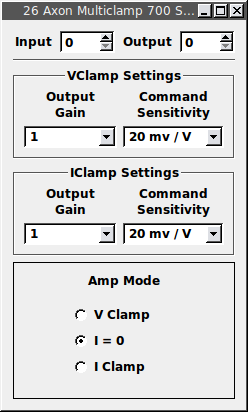
\includegraphics[width=2in]{axon700.png}
\caption[axon700]{This is the control module for Axon Multiclamp 700 Series Commander.}
\end{center}
\end{figure}

The VClamp and IClamp settings of the module must match the amplifier settings set by the user through the Axon software. The mode must also correspond to Axon software, unless the module is being to control the mode. Mode control is done through the amplifier's mode input located on the front of the amplifier.

output(0) - "Mode Telegraph" : Outputs an analog voltage signal to the amplifier through the mode telegraph, allowing the module to control the mode of the amplifier. The "Ext" box must be checked on the Axon software, located next to the mode.